\chapter{Measurement}

\section{Simple vs Aggregate Measurement}
\subsection*{Scenario Objective}


This scenario demonstrates how to represent measurements within the context of the \textbf{BFO/IOF ontology}. It then also represents how to capture processing simple measurements to get an aggregate result (such as doing an average). 

\subsection*{Key Points}
\begin{itemize}
    \item This pattern highlights the connection between a measurement and the attribute that is being measured
    \item The pattern demonstrates how measurements are processed and introduces a distinction between measured data and process data and its association with an attribute
    \item For the examples in hand QUDT is used for representing units according to the guide x. It should be noted that using QUDT is not normative for the IOF
\end{itemize}

\subsection*{General Pattern Description}
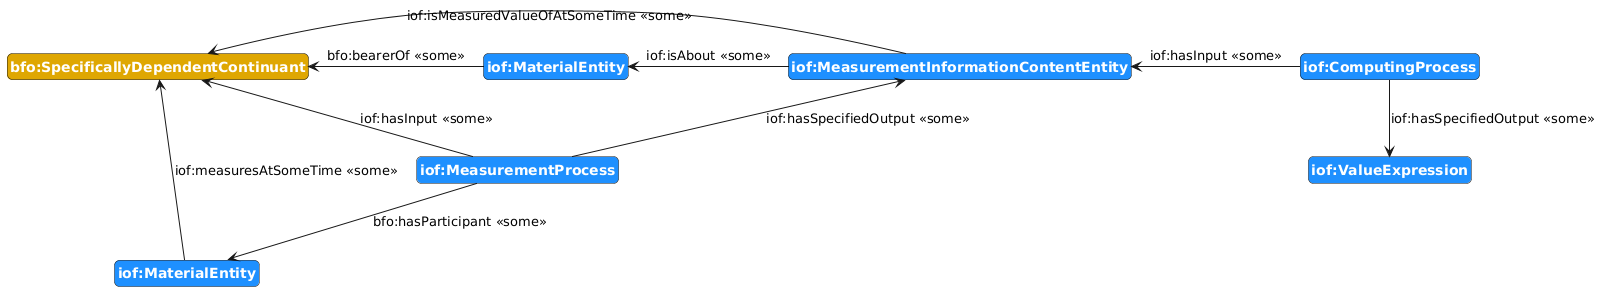
\includegraphics[scale=0.3]{scenarios/measurements/image/measurement_aggregate_general.png}

\subsection{Use case: Measuring protein concentration with a  Bicinchoninic Acid (BCA) Assay}
Within a laboratory environment protein concentration during batch purification is typically measured by using the BCA assay. The assay is based on a colorimetric detection method, where the analyte reacts with a specific reagent to produce a quantifiable color change. The absorbance of the reaction product is measured at a defined wavelength using a spectrophotometer, with the signal intensity correlating to the analyte concentration according to a pre-established standard curve.  The details of converting absorbance into concentration are excluded in the pattern given here. To capture this conversion ontologically the reader should take a look at [placeholder UC] 

Each concentration measurement is performed in triplicate to ensure accuracy, reproducibility, and compliance with quality control standards. Three independent aliquots (samples) are analyzed under identical experimental conditions, with results recorded separately. The final reported concentration value is then derived from the mean of these replicates. It should be noted that in addition to the mean the standard deviation is reported. However, this is outside of the scope of the pattern. For representing standard deviation the reader can look at [placeholder]

\subsubsection*{Use-Case Pattern Description}

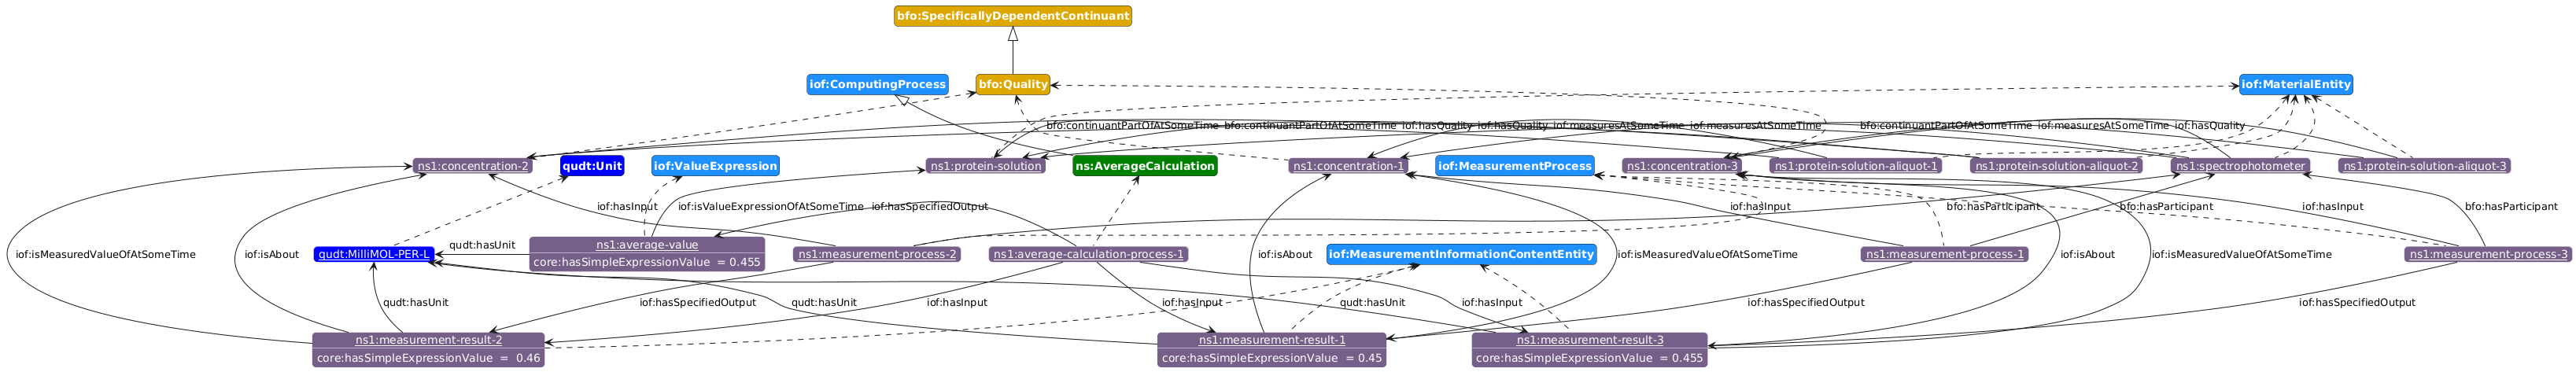
\includegraphics[scale=0.15]{scenarios/measurements/image/measurement_aggregate_usecase1.png}
\subsubsection{Actors}
The primary actors involved in this use case include:
\begin{itemize}[noitemsep]
    \item \textbf{Spectrophotometer (ns1:spectrophotometer):} A material entity that participates in the measurement process by performing the actual measurement of the protein solution.
    \item \textbf{Measurement Process (ns1:measurement-process-1):} The process responsible for recording the protein concentration from the sample. (Note: Additional measurement processes, such as \texttt{ns1:measurement-process-2} and \texttt{ns1:measurement-process-3}, follow the same pattern.)
    \item \textbf{Protein Solution Aliquot (ns1:protein-solution-aliquot-1):} The sample containing the protein solution that is subject to measurement.
    \item \textbf{Concentration Quality (ns1:concentration-1):} The quality attribute of the protein solution representing the measured concentration.
    \item \textbf{Measurement Result (ns1:measurement-result-1):} The output produced by the measurement process, capturing the numerical concentration value along with its unit.
    \item \textbf{Computing Process (Average Calculation) (ns1:average-calculation-process-1):} The process that aggregates multiple measurement results to compute an average concentration value.
    \item \textbf{Average Value (ns1:average-value):} The computed average concentration value, representing a more reliable measurement of the protein concentration.
    \item \textbf{Protein Solution (ns1:protein-solution):} The overall material entity to which the measurement and computed average are associated.
\end{itemize}



\subsubsection{Process Steps}
The process unfolds in the following steps:
\begin{enumerate}[noitemsep]
    \item \textbf{Measurement Execution:}
    \begin{itemize}[noitemsep]
        \item The spectrophotometer (\texttt{ns1:spectrophotometer}) measures the protein concentration of the aliquot (\texttt{ns1:protein-solution-aliquot-1}).
        \item The measurement process (\texttt{ns1:measurement-process-1}) records a result (\texttt{ns1:measurement-result-1}) that includes a concentration value (e.g., "0.45") and its unit (\texttt{qudt:MilliMOL-PER-L}).
    \end{itemize}
    \item \textbf{Data Association:}
    \begin{itemize}[noitemsep]
        \item The measurement result (\texttt{ns1:measurement-result-1}) is linked to the concentration quality (\texttt{ns1:concentration-1}) of the protein solution.
        \item The result is annotated with the appropriate unit of measure, ensuring data consistency.
    \end{itemize}
    \item \textbf{Average Calculation:}
    \begin{itemize}[noitemsep]
        \item A computing process (\texttt{ns1:average-calculation-process-1}) aggregates multiple measurement results.
        \item An average value (\texttt{ns1:average-value}) is computed, offering a reliable estimate of the protein concentration.
        \item The computed average is associated with the overall protein solution (\texttt{ns1:protein-solution}).
    \end{itemize}
\end{enumerate}

By following this pattern, the protein solution retains references to both individual measurements and the computed average, ensuring traceability. 


\subsubsection*{Use-Case Example Data}
Three rows of a CSV table are given bellow where each row constitutes an id of the material from which the aliquots are taken from. The concentration of each aliquot and finally the aggregate measurement. 
Concentrations are reported in g/l.

\begin{table}[ht]
\centering
\caption{Triplicate Measurement Data after a purification step (Concentrations in mmol/l)}
\label{tab:triplicate_measurements}
\begin{tabular}{lccc c}
\toprule
\textbf{Material ID} & \textbf{Aliquot 1 (mmol/l)} & \textbf{Aliquot 2 (mmol/l)} & \textbf{Aliquot 3 (mmol/l)} & \textbf{Aggregate (mmol/l)} \\
\midrule
ID001 & 0.45 & 0.46 & 0.455 & 0.455 \\
ID002 & 0.50 & 0.52 & 0.51  & 0.51  \\
ID003 & 0.42 & 0.43 & 0.425 & 0.425 \\
\bottomrule
\end{tabular}
\end{table}

\subsubsection*{Data Mapping Description}

\begin{verbatim}
INSERT DATA {
# Classes
   ns:AverageCalculation rdfs:subClassOf iof:ComputingProcess .  
  # Individuals
  ns1:measurement-process-1 a iof:MeasurementProcess .
  ns1:measurement-result-1 a iof:MeasurementInformationContentEntity .
  ns1:protein-solution-aliquot-1 a iof:MaterialEntity .
  ns1:concentration-1 a bfo:Quality .
  ns1:spectrophotometer a iof:MaterialEntity .
  ns1:average-calculation-process-1 a ns:AverageCalculation .
  ns1:average-value a iof:ValueExpression .
  ns1:protein-solution a iof:MaterialEntity .
  qudt:MilliMOL-PER-L a qudt:Unit .
  
  # Relationships
  ns1:measurement-process-1 iof:hasSpecifiedOutput ns1:measurement-result-1 .
  ns1:measurement-process-1 iof:hasInput ns1:concentration-1 .
  ns1:measurement-process-1 bfo:hasParticipant ns1:spectrophotometer .
  
  ns1:spectrophotometer iof:measuresAtSomeTime ns1:concentration-1 .
  ns1:protein-solution-aliquot-1 iof:hasQuality ns1:concentration-1 .
  ns1:measurement-result-1 iof:isMeasuredValueOfAtSomeTime ns1:concentration-1 .
  ns1:measurement-result-1 iof:isAbout ns1:concentration-1 .
  
  ns1:measurement-result-1 qudt:hasUnit qudt:MilliMOL-PER-L .
  ns1:measurement-result-1 core:hasSimpleExpressionValue "0.45" .
  
  ns1:average-calculation-process-1 iof:hasInput ns1:measurement-result-1 .
  ns1:average-calculation-process-1 iof:hasSpecifiedOutput ns1:average-value .
  ns1:average-value iof:isValueExpressionOfAtSomeTime ns1:protein-solution .
  ns1:average-value core:hasSimpleExpressionValue "0.455" .
  ns1:average-value qudt:hasUnit qudt:MilliMOL-PER-L .
  
  ns1:protein-solution-aliquot-1 bfo:continuantPartOfAtSomeTime ns1:protein-solution .
  
  # Additional measurement instances (measurement 2 & 3 follow the same pattern)
  ns1:measurement-process-2 a iof:MeasurementProcess .
  ns1:measurement-result-2 a iof:MeasurementInformationContentEntity .
  ns1:protein-solution-aliquot-2 a iof:MaterialEntity .
  ns1:concentration-2 a bfo:Quality .
  
  ns1:measurement-process-2 iof:hasSpecifiedOutput ns1:measurement-result-2 .
  ns1:measurement-process-2 iof:hasInput ns1:concentration-2 .
  ns1:measurement-process-2 bfo:hasParticipant ns1:spectrophotometer .
  
  ns1:spectrophotometer iof:measuresAtSomeTime ns1:concentration-2 .
  ns1:protein-solution-aliquot-2 iof:hasQuality ns1:concentration-2 .
  ns1:measurement-result-2 iof:isMeasuredValueOfAtSomeTime ns1:concentration-2 .
  ns1:measurement-result-2 iof:isAbout ns1:concentration-2 .
  
  ns1:measurement-result-2 qudt:hasUnit qudt:MilliMOL-PER-L .
  ns1:measurement-result-2 core:hasSimpleExpressionValue "0.46" .
  
  ns1:protein-solution-aliquot-2 bfo:continuantPartOfAtSomeTime ns1:protein-solution .
  
  ns1:measurement-process-3 a iof:MeasurementProcess .
  ns1:measurement-result-3 a iof:MeasurementInformationContentEntity .
  ns1:protein-solution-aliquot-3 a iof:MaterialEntity .
  ns1:concentration-3 a bfo:Quality .
  
  ns1:measurement-process-3 iof:hasSpecifiedOutput ns1:measurement-result-3 .
  ns1:measurement-process-3 iof:hasInput ns1:concentration-3 .
  ns1:measurement-process-3 bfo:hasParticipant ns1:spectrophotometer .
  
  ns1:spectrophotometer iof:measuresAtSomeTime ns1:concentration-3 .
  ns1:protein-solution-aliquot-3 iof:hasQuality ns1:concentration-3 .
  ns1:measurement-result-3 iof:isMeasuredValueOfAtSomeTime ns1:concentration-3 .
  ns1:measurement-result-3 iof:isAbout ns1:concentration-3 .
  
  ns1:measurement-result-3 qudt:hasUnit qudt:MilliMOL-PER-L .
  ns1:measurement-result-3 core:hasSimpleExpressionValue "0.455" .
  
  ns1:protein-solution-aliquot-3 bfo:continuantPartOfAtSomeTime ns1:protein-solution .
}

\end{verbatim}

\subsubsection*{Data Validation}

\begin{verbatim}
# Shape for MeasurementProcess
ns:MeasurementProcessShape a sh:NodeShape;
    sh:targetClass iof:MeasurementProcess;
    sh:property [
        sh:path iof:hasSpecifiedOutput;
        sh:class iof:MeasurementInformationContentEntity;
        sh:minCount 1;
    ];
    sh:property [
        sh:path iof:hasInput;
        sh:class bfo:Quality;
        sh:minCount 1;
    ];
    sh:property [
        sh:path bfo:hasParticipant;
        sh:class iof:MaterialEntity;
        sh:minCount 1;
    ].

# Shape for MeasurementInformationContentEntity
ns:MeasurementResultShape a sh:NodeShape;
    sh:targetClass iof:MeasurementInformationContentEntity;
    sh:property [
        sh:path iof:isMeasuredValueOfAtSomeTime;
        sh:class bfo:Quality;
        sh:minCount 1;
        sh:maxCount 1;
    ];
    sh:property [
        sh:path iof:isAbout;
        sh:class bfo:Quality;
        sh:minCount 1;
    ];
    sh:property [
        sh:path qudt:hasUnit;
        sh:class qudt:Unit;
        sh:minCount 1;
    ];
    sh:property [
        sh:path core:hasSimpleExpressionValue;
        sh:datatype xsd:string;
        sh:minCount 1;
    ].

# Shape for Average Calculation Process
ns:AverageCalculationShape a sh:NodeShape;
    sh:targetClass iof:ComputingProcess;
    sh:property [
        sh:path iof:hasInput;
        sh:class iof:MeasurementInformationContentEntity;
        sh:minCount 1;
    ];
    sh:property [
        sh:path iof:hasSpecifiedOutput;
        sh:class iof:ValueExpression;
        sh:minCount 1;
        sh:maxCount 1;
    ].

# Shape for ValueExpression
ns:ValueExpressionShape a sh:NodeShape;
    sh:targetClass iof:ValueExpression;
    sh:property [
        sh:path iof:isValueExpressionOfAtSomeTime;
        sh:class iof:MaterialEntity;
        sh:minCount 1;
    ];
    sh:property [
        sh:path core:hasSimpleExpressionValue;
        sh:datatype xsd:string;
        sh:minCount 1;
    ];
    sh:property [
        sh:path qudt:hasUnit;
        sh:class qudt:Unit;
        sh:minCount 1;
    ].

\end{verbatim}
\section{Unitless measurements}
count, percentage. ratio

\section{Multiple measurements of the same object at the same time}
different measurement processes 

\subsection*{Scenario Objective}

This scenario demonstrates how to represent measurements conducted on different attributes of the same material entity within the context of the \textbf{BFO/IOF ontology}.

\subsection*{Key Points}
\begin{itemize}
    \item This pattern demonstrates how to capture and represent various attributes (e.g., physical, chemical, mechanical) measured on the same material entity.
    \item The pattern demonstrates the temporal coincidence of different measurements.
     \item The pattern highlights how measurements of various attributes can be traced back to the same material entity by using the IOF Core
\end{itemize}
\subsection{Use case: Measurement of temperature and pH during fermentation}
This use case describes a scenario in which temperature and pH measurements are captured during a fermentation process. The temperature sensor records thermal conditions critical for maintaining optimal enzymatic reactions and microbial activity, as deviations can lead to inefficient fermentation or undesirable by-products. Concurrently, the pH sensor monitors the acidity or alkalinity of the fermenting mixture, providing essential insights into the chemical environment that directly affects enzyme functionality, product quality or overall process efficiency.
This use case will focus on capturing a particular (discrete) measurement of temperature and pH. In practice, both attributes are monitored and captured continuously. For the details on how continuous measurements are captured the reader should look at the time-series measurement usecase.

\section{Measurements of the same attribute by using different instruments}

\subsection*{Scenario Objective}

This scenario demonstrates how to represent measurements conducted on same attribute but with different measurement instruments within the context of the \textbf{BFO/IOF ontology}.
\subsection{Use case: Measurement of glucose by Raman spectroscopy and a glucose sensor during fermentation}
In this biomanufacturing use case, glucose concentration—a key parameter for controlling cell culture metabolism—is measured using both Raman spectroscopy and a traditional electrochemical glucose sensor to ensure accuracy and process robustness. The Raman spectrometer provides real-time, non-invasive monitoring of glucose levels by analyzing molecular vibrational signatures, offering a continuous and label-free measurement method. In parallel, an electrochemical glucose sensor, based on enzymatic oxidation, provides direct, quantitative readings through periodic offline sampling. The Raman data enables trend analysis and predictive modeling, while the electrochemical sensor serves as a validation tool to confirm Raman-derived values and detect potential spectral interferences. 
This hybrid measurement approach enhances confidence in glucose monitoring, ensuring precise feed control strategies that optimize cell growth, productivity, and overall biomanufacturing efficiency.

\section{Time-series measurement}
(process characteristics)

\section{uncertainty, range of values}
if time permits

